\chapter{Machine Learning Models}
\section{Overview}

\section{Decision Trees}
Classification trees are used to separate the categories (default, non-default) as best as possible using explanatory factors. The split is determine by maximising the homogeneity of the resulting subgroups (branch). For numeric variables, the algorithm calculates the measure for each possible threshold, while for categorical variables, it determines the value for each possible split. This step is repeated until a stopping condition is met and the final subgroup is called leaf. To avoid overfitting, the Decision Tree may be "pruned", where some branches are removed. The preliminary decision tree is applied on a separate data set, i.e. the validation sample, and to improve its performance, redundant splits are cut off. An example of a decision tree and the pruning process is visible in Fig. \ref{fig:ml_dectree}. A Separate validation should then be performed on a third test data set, since the validation sample became part of the modelling process. 

\begin{figure}[H]
	\centering
	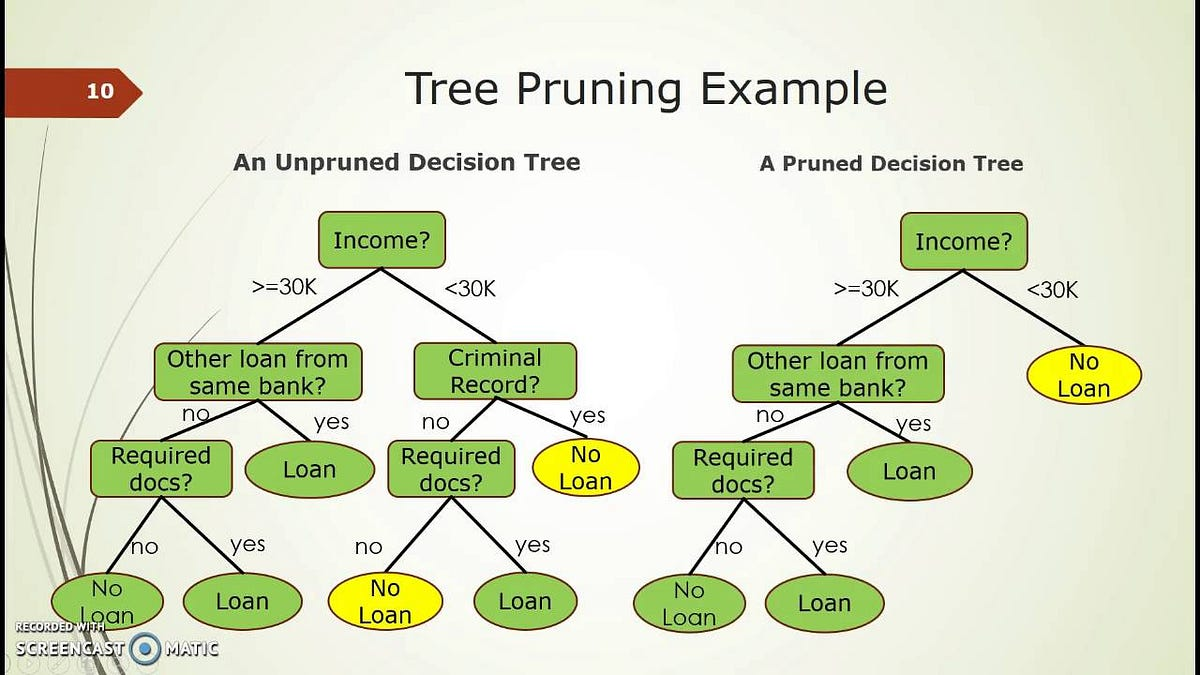
\includegraphics[width=0.625\textwidth]{./ML__DecTree.jpg}
    \caption{Decision Tree incl. Pruning}
    \label{fig:ml_dectree}
\end{figure}

Examples for stopping conditions are that the resulting subgroups are homogeneous, no significant improvement is detected, the minimum leafsize is reached, maximum splits are performed or maximum depth of the tree is achieved. The estimated PD is the average default rate per leaf and each terminal node can be classified into default or non-default using a defined threshold. Popular statistics to measure the homogeneity are Gini index, Kolmogorov-Smirnov statisic or Entropy index. The Gini index assumes a value between 0 and 1, where 0 means complete purity, 0.5 represents an equal distribution of all classes and 1 shows a random distribution across all classes. The formula is given in \ref{eq:ml_gini}. Decision trees usually perform worse than logistic regression models and are rather used to assess the best variables or segmentation possibilities. 

\begin{equation}
GINI = \sum_{i=1}^{n}  p_i \times (1 - p_i) \label{eq:ml_gini}
\end{equation}
where:
\begin{conditions}
 n  	& number of unique classes in variable \\
 p_{i}  & proportion of observations in class n
\end{conditions}

\subsection{Boosted Decision Trees and Random Forests} 
Boosted Decision Trees (BDT), also known as Gradient Boosted Decision Trees combine decision trees with boosting techniques to achieve higher predictive performance. This algorithm iteratively build decision trees, placing more weight on misclassified observations in each iteration, resulting in a strong ensemble model, seen in Fig. \ref{fig:ml_bdt}. BDT are able to capture complex interactions and non-linear relationships in PD modelling. 

\begin{figure}[H]
	\centering
	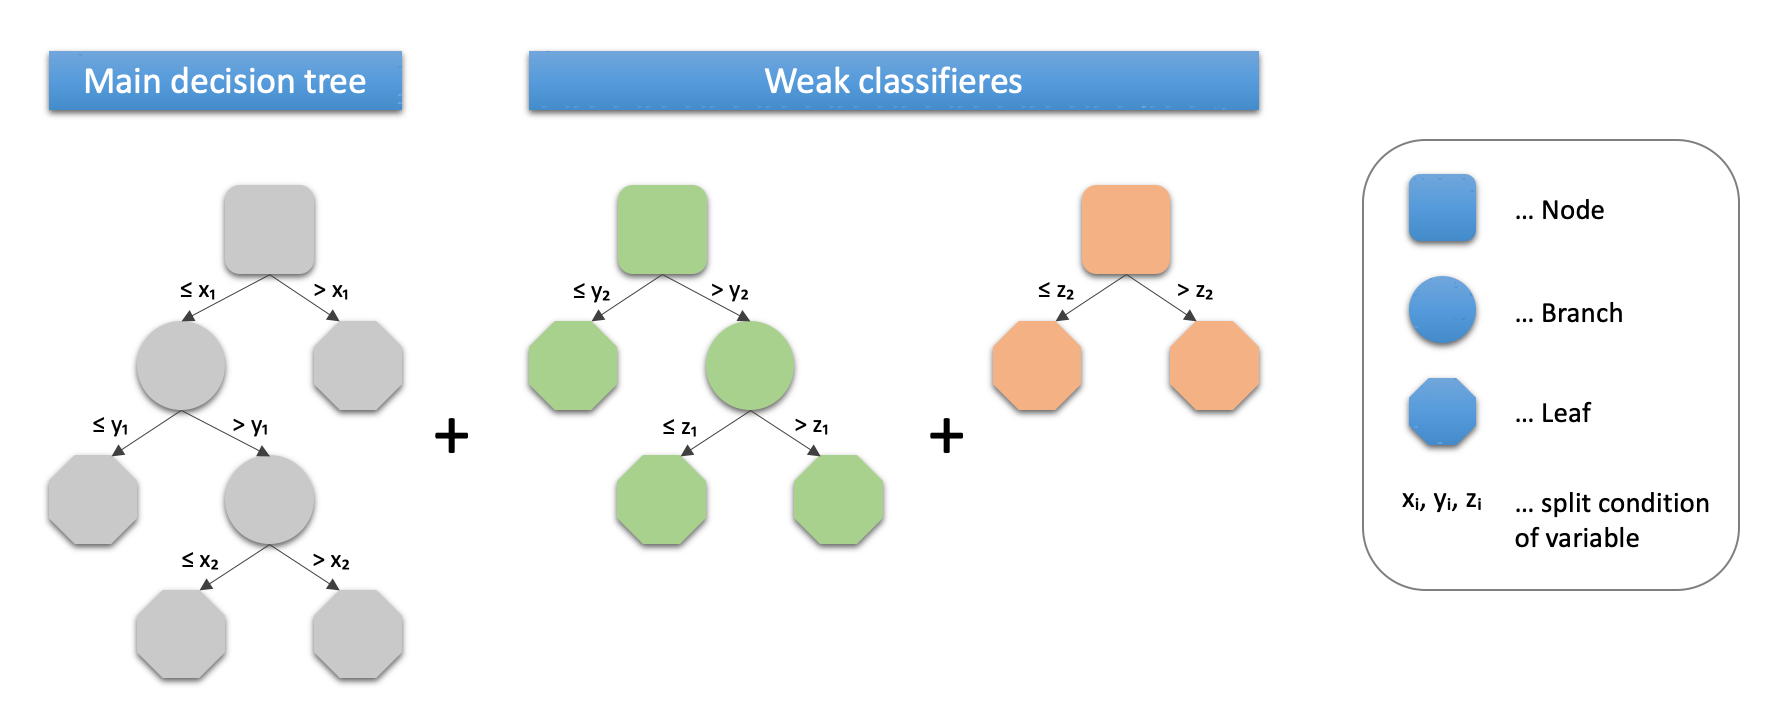
\includegraphics[width=0.625\textwidth]{./ML__BDT.png}
    \caption{Boosted Decision Tree}
    \label{fig:ml_bdt}
\end{figure}

Random forests are an ensemble learning method that combines multiple decision trees to make predictions. However, unlike boosted decision trees, random forests build each tree independently, without sequential corrections (Fig. \ref{fig:ml_ranforest}). This approach reduce the risk of overfitting and the variance of predictions. Random forests are known for their robustness, scalability, and ability to handle high-dimensional data.

\begin{figure}[H]
	\centering
	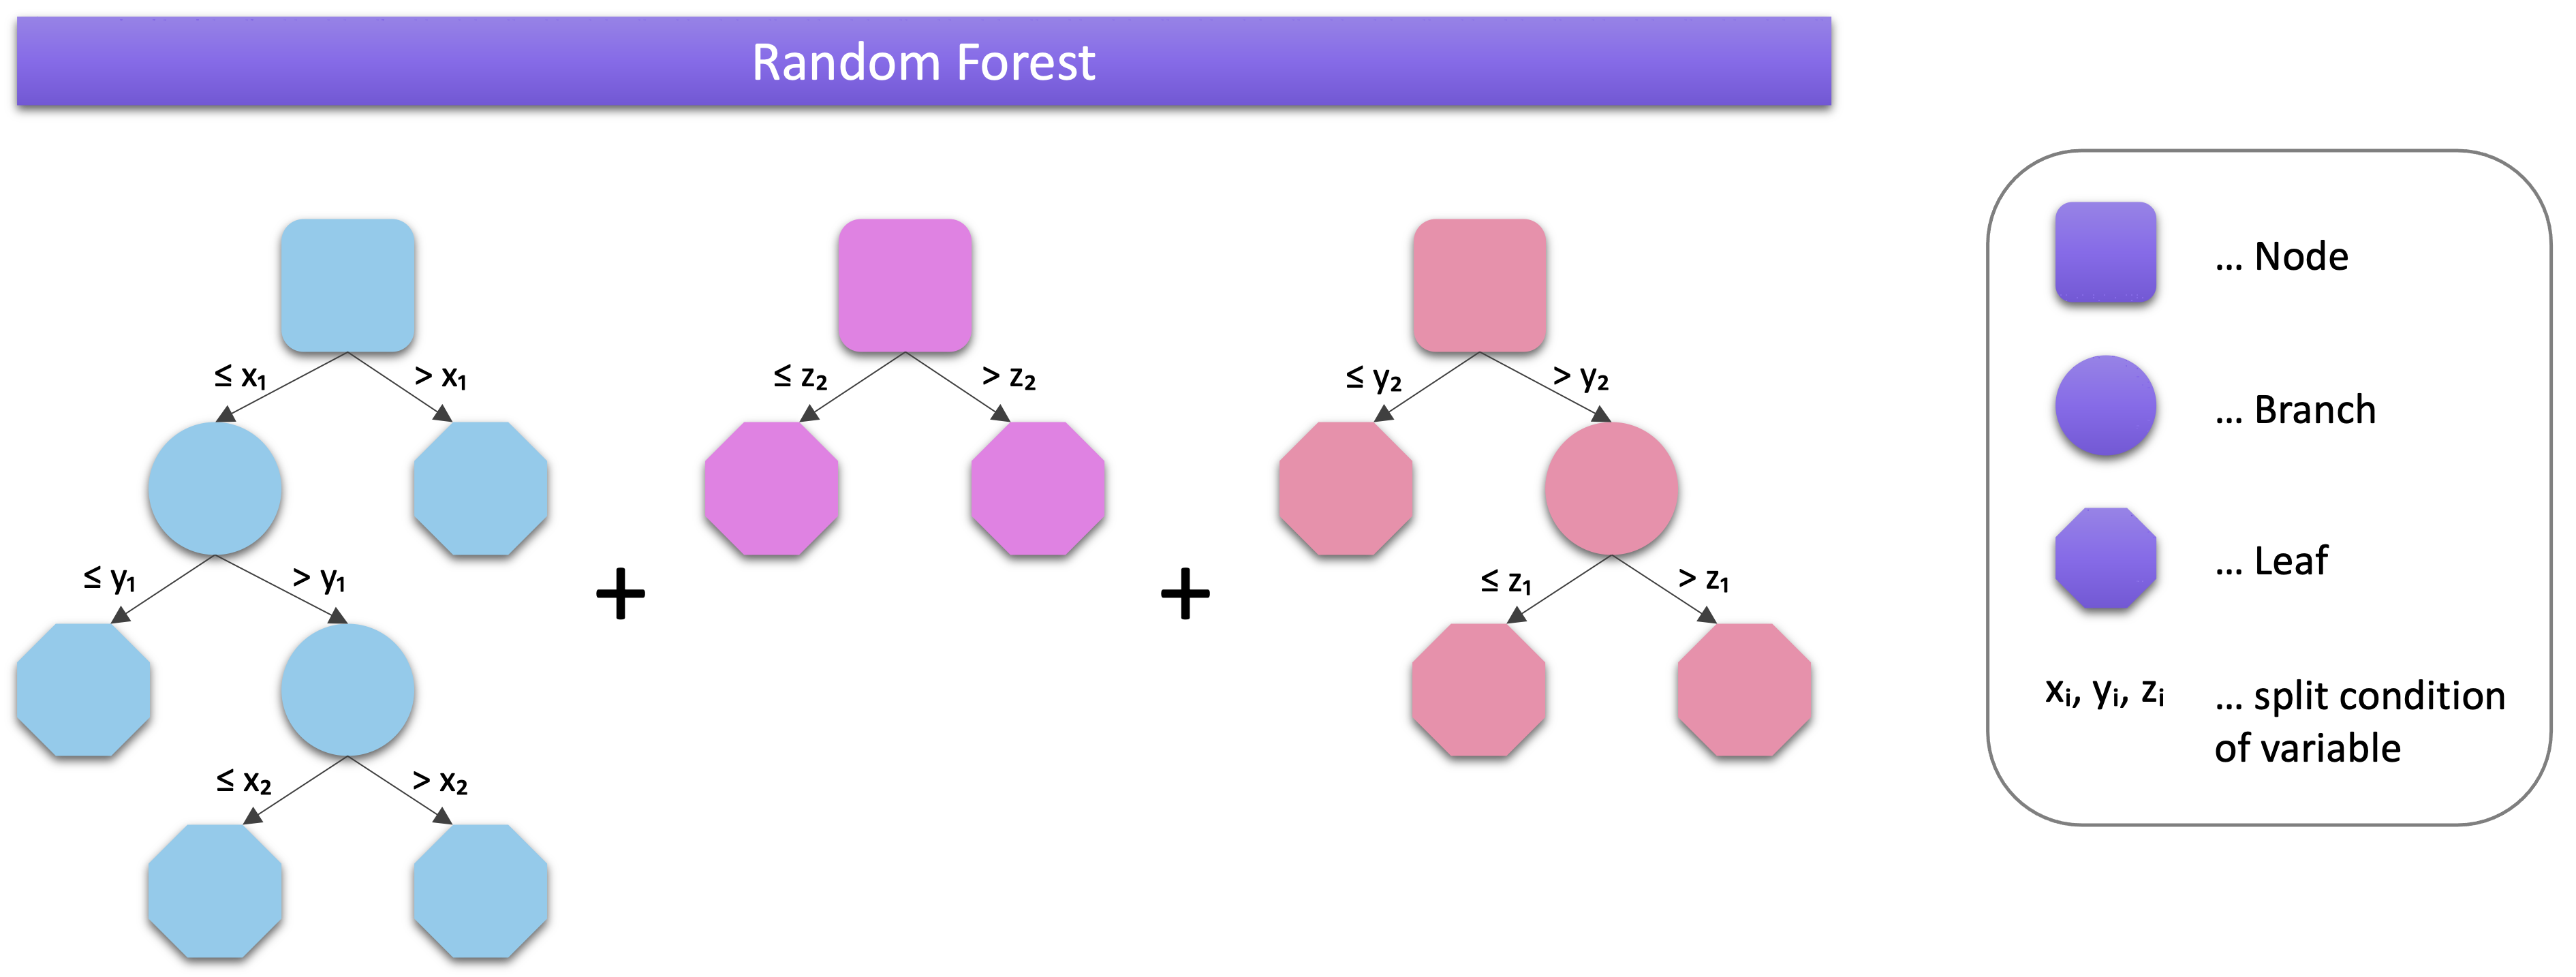
\includegraphics[width=0.625\textwidth]{./ML__Random_forest.png}
    \caption{Random Forest}
    \label{fig:ml_ranforest}
\end{figure}

\section{Other models}

\subsection{Neural Networks}
Neural networks, inspired by the structure and function of the human brain, can learn intricate patterns and nonlinear relationships in data. They consist of multiple layers of interconnected nodes, also called neurons, where each neuron is assigned a simple computation and use activation functions to pass along a value. The result of the model is a numerical or classification value. Commonly used activation functions are logistic function, threshold function or tangent hyperbolic function, listed in Eq. \ref{fig:ml_logfunc} - \ref{fig:ml_tanhfunc}. 

The first and last layer is called the input and output layer respectively, and the layers in-between are hidden layers. An illustration is visible in Figure \ref{fig:ml_neurnet}. Due to the virtually endless possibility of configurations, there is a possibility of over-parametrization, especially with increasing number of hidden layers and nodes, also called deep neural networks. With the ongoing advancements in computational power and data collection capabilities, neural network algorithms have become highly successful in various AI domains.

\begin{figure}[H]
	\centering
	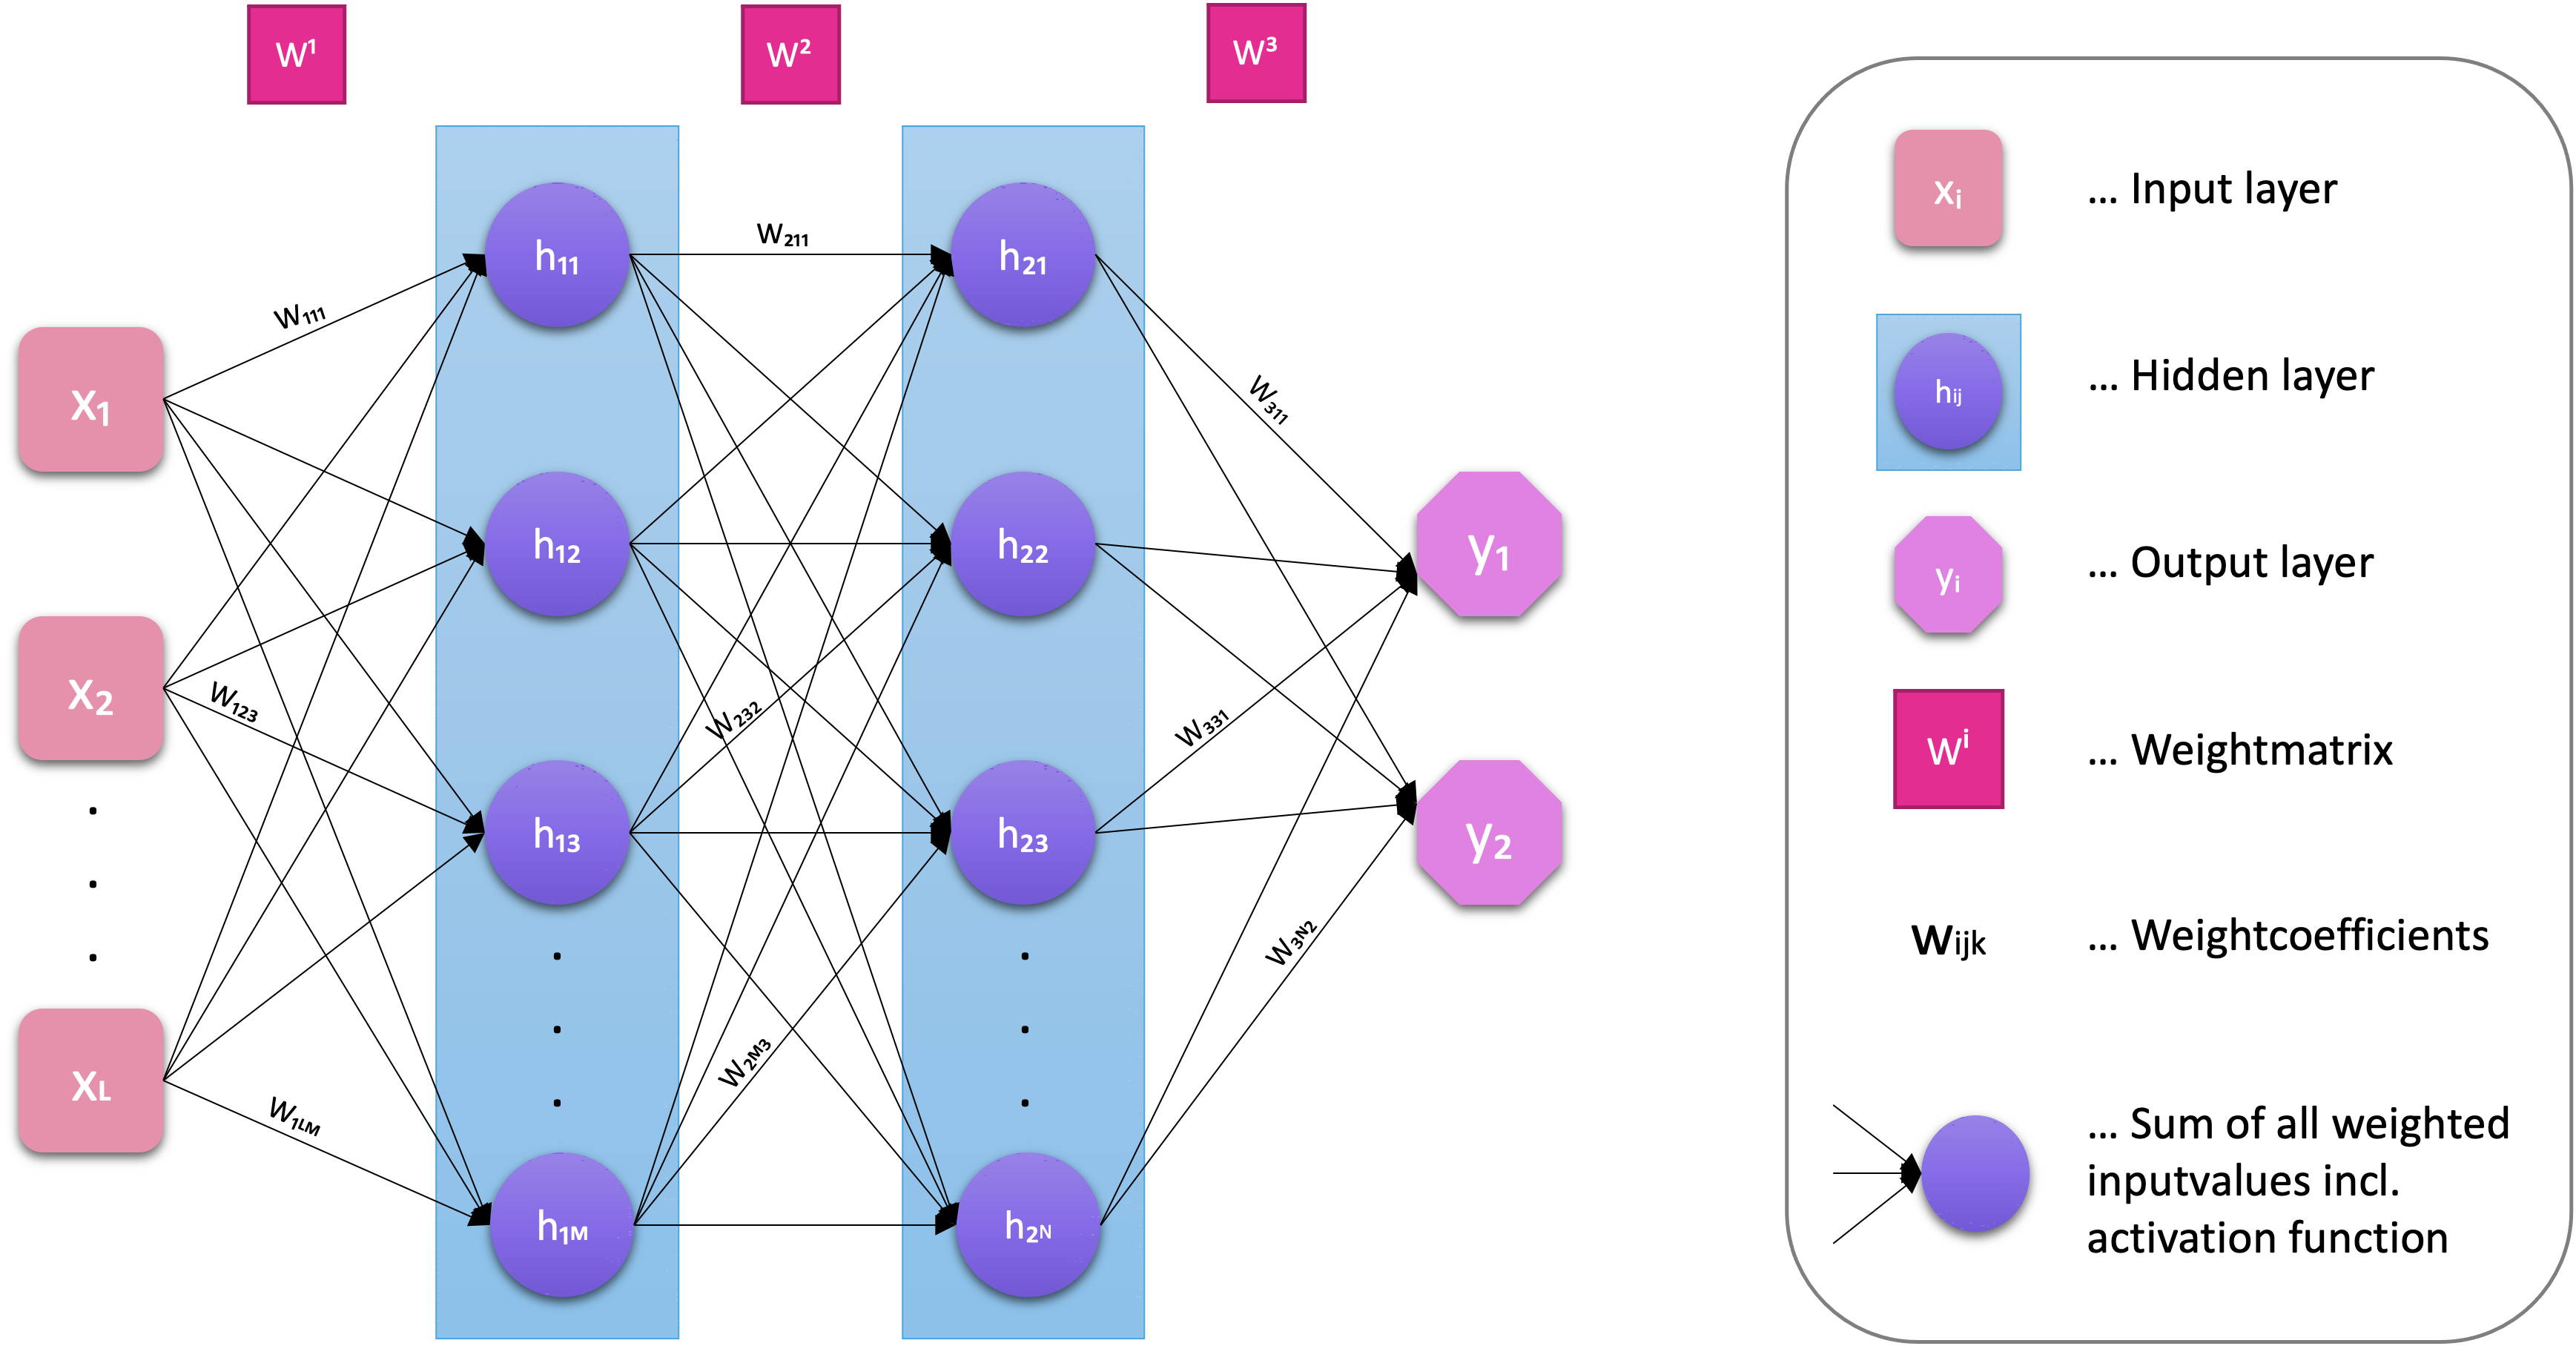
\includegraphics[width=0.625\textwidth]{./ML__MLP.png}
    \caption{Neural Network}
    \label{fig:ml_neurnet}
\end{figure}

\subsection{k-Nearest Neighbour}
\label{sec:kNN}
Using a data set with explanatory factors and known default events, the unknown PD of a new data entry can be determined by taking the nearest data points determined via their risk factors and calculating the average default rate of the new data point. For the definition of distance the Euclidean metric or Manhattan Distance as defined in formula \ref{fig:ml_eucldist} and \ref{fig:ml_manhdist} can be used. The Euclidean distance measures the straight-line distance between two points, while the Manhattan distance is the sum of the absolute differences between two points in a space, where it is only allowed to move along coordinate axes. The number of nearest neighbours k is a hyper-parameter. Advantages of this model is the simple approach and the possibility to dynamically update new and outdated data entries and, if k is set as a low number, individual scorings can be viewed manually by a credit analyst. 

\subsection{Ensamble models}